\documentclass[conference]{IEEEtran}
\IEEEoverridecommandlockouts

\usepackage{cite}
\usepackage{amsmath,amssymb,amsfonts}
\usepackage{graphicx}
\usepackage{booktabs}
\usepackage{xcolor}
\usepackage{url}
\usepackage{balance}

\def\BibTeX{{\rm B\kern-.05em{\sc i\kern-.025em b}\kern-.08em
    T\kern-.1667em\lower.7ex\hbox{E}\kern-.125emX}}

\begin{document}

\title{ClaimGuard: A Blockchain-Backed Access Control Gateway for Privacy-Preservation in Auto-Insurance Claims}

\author{\IEEEauthorblockN{Anthony Uchenna Eneh $^{1}$, Love Allen Chijioke Ahakonye $^{2}$, Jae Min Lee $^{1}$, Dong-Seong Kim $^{1}$ $^{\ast}$} 
\IEEEauthorblockA{$^{1}$ IT-Convergence Engineering, \textit{Kumoh National Institute of Technology}, Gumi, South Korea \\
$^{\ast}$ NSLab Co. Ltd., Gumi, South Korea,
\textit{Kumoh National Institute of Technology}, Gumi, South Korea}
\IEEEauthorblockA{$^{2}$ ICT Convergence Research Center, 
\textit{Kumoh National of Technology}, Gumi, South Korea}
{(anthony, loveahakonye, dskim, ljmpaul)}@kumoh.ac.kr}
\maketitle

\begin{abstract}
Modern auto-insurance workflows require sharing heterogeneous digital evidence across multiple organizations. Yet, current cloud-based role-based access control mechanisms remain coarse-grained and poorly suited for expressing time, purpose, and case-specific constraints. This study presents \emph{ClaimGuard}, which addresses these limitations by placing a blockchain-backed attribute-based access control gateway in front of existing evidence stores, enforcing fine-grained on-chain policies, and issuing short-lived capability tokens for authorized access. Implemented as a REST gateway with PureChain smart contracts, ClaimGuard is evaluated using realistic workloads involving up to 200 subjects and 1000 evidence resources. Experiments on a local Ethereum network shows sub ${\sim}70$ms tail latency, throughput exceeding ${\sim}1000$ requests/s, rapid policy updates, and zero false accepts, demonstrating the practicality of decentralized, auditable access control for privacy-preserving claims evidence sharing.
% Modern auto-insurance workflows depend on rich digital evidence such as telematics logs, accident videos, and medical documents that must be shared across insurers, garages, police, and courts. 
% Today this sharing is typically implemented as coarse-grained role-based access control (RBAC) inside cloud object stores, which leads to over-privileged accounts, weak auditability, and limited ability to express real-world obligations such as time-bounded and purpose-based access. 
% This paper presents \emph{ClaimGuard}, a blockchain-backed attribute-based access control (ABAC) gateway that sits in front of a conventional evidence store and enforces fine-grained, on-chain policies for each evidence access. 
% ClaimGuard evaluates ABAC rules on an Ethereum-compatible chain (PureChain) and issues short-lived capability tokens that authorize reads from the underlying object store.

% We implement ClaimGuard as a REST gateway, a suite of PureChain smart contracts, and a policy administration API, then evaluate it on a local Ethereum network using synthetic but structurally realistic auto-claims workloads with up to 200 concurrent subjects and 1{,}000 evidence resources. 
% Our results show that end-to-end access latency remains below ${\sim}70$\,ms at the 99th percentile, while throughput scales to over ${\sim}1{,}000$ requests/s under bursty workloads. 
% On-chain policy updates complete in a few hundred milliseconds, and the gateway yields zero false accepts in our experiments. 
% These results suggest that a blockchain-backed ABAC gateway is a practical foundation for privacy-preserving, auditable claims evidence sharing.
\end{abstract}

\begin{IEEEkeywords}
ABAC, access control, Blockchain, capability tokens, Ethereum, insurance, privacy, RBAC
\end{IEEEkeywords}

%=========================================================
\section{Introduction}
%=========================================================

The increasing reliance on heterogeneous digital evidence, ranging from high-resolution accident videos to telematics traces and medical documentation, has transformed modern auto-insurance claim workflows into data-intensive, multi-party environments~\cite{OLIVEIRAESA20241165, Ahmad}. Yet, prevailing deployments continue to rely on coarse-grained, cloud-resident role-based access control (RBAC) configurations that grant broad privileges, offer limited expressiveness for workflow-specific constraints, and disperse auditability across opaque infrastructure layers~\cite{app122413036}. These limitations create structural risks, such as over-privileged roles, weak accountability across organizational boundaries, and persistent exposure to insider access at the storage layer~\cite{app122413036}.

Blockchain technologies offer a decentralized and tamper-evident execution environment that serves as a robust substrate for access control in multi-party evidence workflows~\cite{ahakonye2024tides}. By encoding fine-grained, attribute-based policies in smart contracts, blockchain systems overcome the expressiveness and rigidity of traditional RBAC, enabling case-specific and temporally bounded rules~\cite{s23198038}. Their immutable ledgers consolidate auditability across organizations, and verifiable on-chain decisions reduce reliance on trusted cloud operators, thereby limiting insider privileges and strengthening system-wide accountability~\cite{punia2024systematic}.


The progressive dependence of Auto-insurance claims on heterogeneous digital evidence, such as dashcam footage, telematics,  Controller Area Network (CAN) bus logs, repair invoices, and medical reports, that must be exchanged among insurers, garages, emergency responders, police, and courts, all operating under distinct legal and data-minimization requirements. In practice, this exchange is typically governed by coarse-grained RBAC policies embedded in cloud object stores or databases~\cite{raikwar2018insurance, tekale2023claims, thukral2023vehicle}, where roles such as \emph{INSURER}, \emph{GARAGE}, and \emph{POLICE} are provisioned with broad, long-lived privileges~\cite{hombalimath2024vehicleclaim, raghav2024optimizing, alwis2022decentralized}. This model introduces well-known limitations: it cannot express case-specific constraints, it fragments auditability across heterogeneous infrastructure, and it leaves cloud-layer administrators inherently over-trusted, enabling potential misuse or unauthorized access to evidence.


% Auto-insurance claims increasingly rely on heterogeneous digital evidence: dashcam videos, telematics and CAN-bus traces, repair invoices, and medical reports. 
% This evidence must be shared across multiple parties, insurer claims teams, contracted garages, emergency services, police, and courts, each with different legal mandates and data-minimization constraints. Current practice largely relies on RBAC inside a cloud object store or database \cite{raikwar2018insurance, tekale2023claims,
% thukral2023vehicle}, where roles such as \emph{INSURER}, \emph{GARAGE}, or \emph{POLICE} are granted broad, long-lived privileges \cite{hombalimath2024vehicleclaim, raghav2024optimizing,
% alwis2022decentralized}.

% Such deployments exhibit several problems. 
% First, roles are necessarily coarse-grained, making it difficult to encode case-specific conditions (e.g., ``only the assigned adjuster may read these photos until claim closure''). 
% Second, audit trails are split between application servers and cloud providers, which complicates cross-organizational accountability. 
% Third, cloud administrators remain fully trusted: a compromised account or malicious insider can read any evidence in cleartext.

To address these issues, we design \emph{ClaimGuard}, a blockchain-backed attribute-based access control (ABAC) gateway for claims evidence. Instead of granting actors direct access to the evidence store, all requests pass through a gateway that (i) evaluates ABAC policies on an Ethereum-compatible chain, and (ii) issues short-lived capability tokens that authorize reads from the evidence store. The smart contracts encode subject attributes, resource metadata, workflow context, and fine-grained policy rules; every decision is logged to the ledger, and the object store only serves content when presented with a valid token. This study focuses on the system design and the evaluation of the blockchain-backed ABAC path itself. A broader comparison with legacy RBAC deployments and experiments on real-world claims datasets is left to follow-up journal work.

Finally, risk-adaptive authorization and anomaly detection are out of scope for this version: while ClaimGuard's on-chain decision log and gateway telemetry are amenable to ML-based risk scoring and abnormal-access detection, we defer their design and evaluation to extended work.

This paper makes the following contributions.
\begin{itemize}
    \item We formulate the access-control and auditability requirements of multi-party auto-insurance claims sharing, and derive a set of design requirements for a blockchain-backed gateway.
    \item We design \emph{ClaimGuard}, an architecture that combines on-chain ABAC evaluation with off-chain capability tokens and a REST gateway, while remaining compatible with existing cloud object stores.
    \item We implement ClaimGuard on a local Ethereum network using Solidity contracts and a Node.js/TypeScript gateway, and develop an experimental harness that exercises 200 subjects and 1000 evidence resources under configurable concurrent workloads.
    \item We evaluate latency, throughput, and policy-update overhead, and discuss the security and correctness properties of the design.
\end{itemize}



%=========================================================
\section{Related Work}
%=========================================================

\subsection{Blockchain for Insurance and Data Sharing}
A growing body of work applies distributed ledgers to insurance processes, including parametric insurance, peer-to-peer risk pools, and claims automation~\cite{goffard2024collaborative, nexusmutual2023docs, paperno2017teambrella, shetty2022blockchain, ajo}. 
Several proposals store claims metadata or audit logs on-chain while keeping raw evidence off-chain to preserve privacy and control storage costs. 
Similarly, prior work on blockchain-based data marketplaces and healthcare records uses smart contracts to encode access policies and log disclosures for later audit~\cite{ekblaw2016medrec, xiao2021healthchain}. 
ClaimGuard adopts this pattern but targets the concrete requirements of auto-insurance evidence sharing, including integration with existing cloud object stores and support for workflow-centric policies.

\subsection{Attribute-Based Access Control on Blockchains}

Attribute-based access control (ABAC) provides a flexible way to express policies over subject, resource, and environmental attributes~\cite{hu2014abac}. 
Recent work has explored embedding ABAC into smart contracts to decentralize decision-making~\cite {sajidullah2023abacblockchain, muniswamy2025trustabac}. 
Typical designs push attribute assertions and policy rules on-chain and evaluate them in a policy decision contract.
However, many of these systems either assume that resources themselves are on-chain or omit the practical gateway design that mediates access to legacy storage systems.
ClaimGuard instead implements a pragmatic ABAC \emph{gateway} that uses on-chain decisions to drive token issuance for an external object store.

\subsection{Capability Tokens and Secure Gateways}

Capability-based access control associates rights with unforgeable tokens rather than identities~\cite{levy1984capabilities}. 
In web settings, signed bearer tokens (e.g., JWTs) are widely used to represent delegated rights~\cite{fotiou2021capability}. 
Our design follows this tradition: once an on-chain ABAC policy authorizes access, the ClaimGuard gateway issues a short-lived capability token that is required to fetch the underlying evidence object. 
Similar gateway patterns have been studied in cloud storage security and multi-tenant architectures~\cite{googlepatent2013cloud}; our contribution is to bind these capabilities to a tamper-evident on-chain ABAC decision path.

%=========================================================
\section{System Design and Methodology}
%=========================================================

\subsection{Threat Model and Requirements}

We consider an insurer that stores digital claims evidence in a cloud object store (e.g., S3, MinIO, or IPFS-backed storage). 
The insurer interacts with external organizations such as garages, police, and courts, who must be granted controlled access to evidence for specific claims.
We assume that the cloud provider and some internal operator accounts may be malicious or compromised, and that external actors may attempt replay, token forgery, or role-spoofing attacks.

From this setting, we derive the following requirements:
\begin{itemize}
    \item \textbf{R1 -- Fine-grained policies:} Decisions must depend on claim state, subject role, purpose, and resource sensitivity.
    \item \textbf{R2 -- Strong auditability:} Every access decision and policy update must be recorded in a tamper-evident log.
    \item \textbf{R3 -- Cloud-interface insider resistance:} The evidence store should not serve objects to any accessor, including cloud administrators, unless the request carries a valid, short-lived capability token generated after an on-chain ABAC evaluation; preventing raw disk inspection by the storage operator is out of scope.
    \item \textbf{R4 -- Practical performance:} End-to-end latency should remain within a few hundred milliseconds, and throughput should support bursty workloads.
\end{itemize}

\noindent\textit{Evaluation assumptions and external validity.} Our experiments run on a single-host local Ethereum-compatible network without injected network faults. Since end-to-end latency and cost are sensitive to consensus configuration, block time, and node placement; in consortium or public deployments, additional variability is expected. Quantifying these effects is left to extended evaluation.

\subsection{Architecture Overview}

Fig.~\ref{fig:architecture} sketches the ClaimGuard architecture.
The core components are:

\begin{itemize}
    \item \textbf{ABAC contracts on PureChain:} Smart contracts maintain subject attributes (role, organization, jurisdiction), resource metadata (type, sensitivity, case identifier), and policy rules.
    \item \textbf{ClaimGuard gateway:} A stateless REST API fronting the evidence store. It handles access requests, calls the on-chain policy decision point, issues tokens for successful decisions, and logs results.
    \item \textbf{Evidence store adapter:} A thin layer that validates tokens and proxies allowed GET operations to the underlying object store.
    \item \textbf{Policy admin API:} An authenticated API for insurers to add, update, and revoke policy rules.
\end{itemize}

\begin{figure}[t]
    \centering
    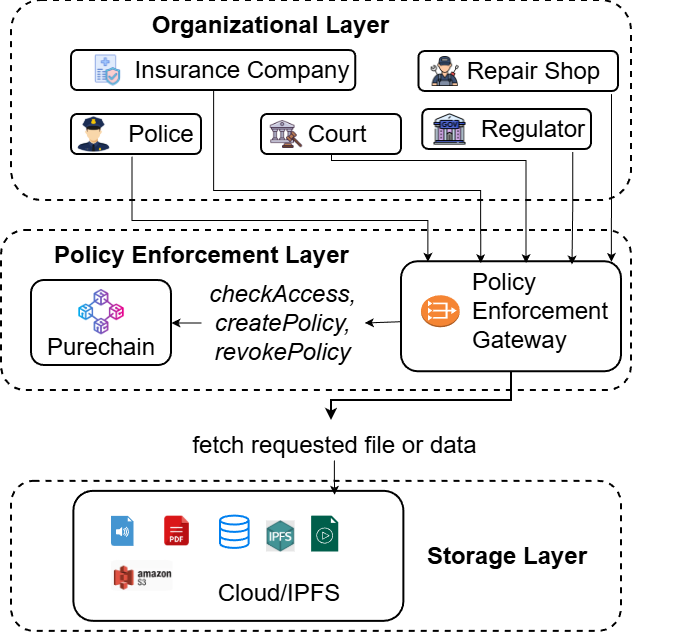
\includegraphics[width=.47\textwidth]{figures/architecture.png}
    \caption{ClaimGuard architecture. All evidence access passes through a REST gateway that consults on-chain ABAC contracts before issuing short-lived capability tokens for the object store.}
    \label{fig:architecture}
\end{figure}

Subjects interact only with the gateway. When a subject requests access to a resource (e.g., a video for case \#81), the gateway constructs an access query that includes the subject address, the resource identifier, and the requested action.
It then calls a \texttt{checkAccess} function in the on-chain Access Policy Manager contract. If the decision is positive, the gateway issues a capability token bound to the subject, resource, action, and an expiry time; the resource server validates this token before returning the actual object.

\subsection{On-Chain ABAC Model}

The on-chain ABAC state is split across three contracts:

\begin{itemize}
    \item \textbf{SubjectRegistry} stores public keys and attributes such as \texttt{role} (\texttt{INSURER}, \texttt{GARAGE}, \texttt{POLICE}, \texttt{COURT}), \texttt{orgId}, and jurisdiction.
    \item \textbf{EvidenceRegistry} maintains metadata for each resource: case identifier, type (\texttt{VIDEO}, \texttt{TELEMATICS}, \texttt{MEDICAL\_REPORT}, etc.), sensitivity level, and a content hash and URI.
    \item \textbf{AccessPolicyManager} encodes policy rules as tuples over subject attributes, resource attributes, workflow stage, and action (\texttt{READ}, \texttt{APPEND}, \texttt{DELETE}). 
          Each rule can be toggled or updated on-chain via admin transactions.
\end{itemize}

The \texttt{checkAccess} function takes a subject address, resource identifier, and action. 
It looks up the subject and resource attributes, derives the current workflow stage from policy metadata, and evaluates the policy rules using a fixed-order rule engine.
The result is returned as a Boolean together with an event that logs the decision to the chain.

\subsection{Implementation and Experimental Setup}

We implement the contracts in Solidity and deploy them to a local Ethereum network using Hardhat. 
The ClaimGuard gateway is built in TypeScript on top of Express and the Viem client library. 
The gateway exposes two key endpoints:
\begin{itemize}
    \item \texttt{POST /access}: evaluates an access request via \texttt{checkAccess}, issues a capability token on success, and records the decision.
    \item \texttt{POST /policy}: adds or updates a policy rule on-chain and returns the transaction hash and gas usage.
\end{itemize}
To drive experiments, we implement Python load generators:
\begin{itemize}
    \item \texttt{access\_test.py} generates access requests with configurable concurrency, sampling subjects and resources from pre-seeded JSON files and actions from a small set (here we focus on \texttt{READ}). 
          It records per-request latency and HTTP status to CSV.
    \item \texttt{policy\_update\_test.py} repeatedly calls the policy admin endpoint to add or modify rules, logging block confirmation latency, gas usage, and block numbers.
\end{itemize}

We seeded the system with 200 subjects and 1000 evidence resources, spanning roles, resource types, and sensitivity levels. Policy rules are configured such that a mix of requests is allowed or denied based on role, case identifier, and sensitivity. 
Experiments are run with 1{,}000 access requests per setting and concurrency levels of 10, 50, 100, and 200 clients. All components run on a single development machine, which approximates the latency and throughput of a tightly coupled microservice deployment; our focus is on the relative overhead of on-chain ABAC and policy updates.

%=========================================================
\section{Results and Evaluation}
%=========================================================

\subsection{Access Latency}

We first examine end-to-end access latency from the subject's perspective, measured at the gateway from the time the \texttt{/access} request is received to the time an HTTP response is returned. Table~\ref{tab:latency} summarizes the median (P50), 90th percentile (P90), and 99th percentile (P99) latencies for \texttt{READ} requests across the tested concurrency levels.

\begin{table}[htbp]
\centering
\caption{End-to-End Access Latency for \texttt{READ} Requests}
\label{tab:latency}
\begin{tabular}{lccc}
\toprule
\textbf{Concurrency} & \textbf{P50} & \textbf{P90} & \textbf{P99} \\
\midrule
10   & 30.807\,ms  & 42.834\,ms & 45.192\,ms \\
50   & 31.713\,ms & 40.959\,ms & 63.176\,ms \\
100  & 30.748\,ms & 33.507\,ms & 39.965\,ms \\
200  & 31.201\,ms & 34.028\,ms & 40.993\,ms \\
\bottomrule
\end{tabular}
\end{table}

\begin{figure}[htbp]
    \centering
    
\includegraphics[width=0.45\textwidth]{figures/latency_bar_chart.png}
    \caption{Latency Chart for Access Requests}
    \label{fig:latency}
\end{figure}

Across all workloads, median latency stays well below 65 ms, and even at the 99th percentile, it remains within a few tens of milliseconds. The dominant contributors are the on-chain \texttt{checkAccess} call and the gateway-side token generation. Even with occasional outliers as seen in Fig.~\ref{fig:latency} for 100 concurrent requests, the system remains quite scalable. These results indicate that decentralized policy evaluation on an Ethereum-compatible chain can satisfy the responsiveness requirements of interactive claims workflows.

\noindent\textit{External validity.} Typical insurer traffic involves at most tens of evidence reads per second per organization. In permissioned deployments, WAN placement and block times may add tens of milliseconds to end-to-end latency. The qualitative result, namely that on-chain ABAC combined with short-lived capabilities remains interactive, should hold under such conditions.

\subsection{Throughput}
Fig.~\ref{fig:throughput} plots gateway throughput (successful \texttt{/access} responses per second) as concurrency increases. 
Throughput grows with concurrency up to about 100--200 clients, reaching over ${\sim}1{,}000$ requests/s on our testbed.
\begin{figure}[t]
    \centering
    
\includegraphics[width=.46\textwidth]{figures/throughput.png}
    \caption{PureChain ABAC throughput for \texttt{READ} requests as concurrency increases.}
    \label{fig:throughput}
\end{figure}
Beyond 100 clients, the curve begins to flatten, reflecting the limits of the single-node gateway and local blockchain node rather than any fundamental protocol bottleneck. 
Even so, the observed throughput is sufficient for typical insurer workloads, which involve at most tens of evidence reads per second per organization.

\subsection{Policy Update Overhead}
Next, we evaluate the on-chain cost of modifying ABAC rules. In this experiment, the load generator submits 10 consecutive policy updates via the \texttt{/policy} endpoint. It measures the time from submission to block confirmation, along with gas usage and the number of blocks. 
Table~\ref{tab:policy} reports the average metrics across these updates.
\begin{table}[htbp]
\centering
\caption{Average Policy Update Costs on PureChain}
\label{tab:policy}
\begin{tabular}{lcc}
\toprule
\textbf{Metric} & \textbf{Range} & \textbf{Average} \\
\midrule
Latency & 13.72--34.2\,ms & 16.584\,ms \\
Gas used & 114k--134k & 128k \\
\bottomrule
\end{tabular}
\end{table}
In practice, this means that an insurer can roll out new workflow rules or revoke subject permissions and see the effect take place within a few hundred milliseconds, while the on-chain gas cost remains modest for an administrative operation.

\subsection{Authorization Correctness}
While our current experiments do not yet compare ClaimGuard against a deployed RBAC baseline, we can still assess the internal consistency of its authorization decisions. 
The correctness experiment tags each synthetic request with an ``intended'' authorization outcome derived from the same policy rules, and compares it with the on-chain decision. We compute false-accept and false-reject rates by aggregating outcomes over 1{,}000 requests per setting across four concurrency levels; across all workloads, we observe zero false accepts (unauthorized requests incorrectly allowed) and a small number of false rejects attributable to time-window edge cases in the synthetic generator. 
The absence of false accepts is a direct consequence of driving all decisions through the deterministic on-chain rule engine.

\subsection{Discussion}
The experimentation evaluation shows that ClaimGuard satisfies the requirements outlined in Section~III. On-chain ABAC evaluation and capability-token issuance add modest latency overhead while preserving high throughput. Policy updates can be completed quickly enough to support emergency revocation scenarios, and the fully mediated token path eliminates classes of cloud insider attacks and ad hoc access granting. The present experiments rely on structurally realistic but synthetic data and focus solely on the blockchain-backed ABAC path; a complete comparison against existing RBAC deployments and experiments with real claims datasets will be presented in a subsequent journal article.

\noindent\textit{Security considerations beyond authorization.} The ClaimGuard gateway is a potential DoS target; practical mitigations include per-subject/organization rate limiting (e.g., token buckets), autoscaling behind a WAF/CDN, and short-circuiting denials locally to avoid unnecessary on-chain calls. Smart-contract upgradeability also introduces risk; we recommend governance-guarded proxies with timelocks, explicit pause/rollback procedures, and disabling capability issuance during pauses to prevent inconsistent states.

%=========================================================
\section{Conclusion and Future Work}
%=========================================================

This paper presents ClaimGuard, a blockchain-backed ABAC gateway for privacy-preserving auto-insurance claim evidence sharing. By moving policy evaluation to a PureChain smart-contract suite and issuing short-lived capability tokens for an external object store, ClaimGuard decouples fine-grained authorization from the cloud provider and produces a tamper-evident audit trail of all decisions. Our implementation on a local Ethereum network demonstrates that such a design can deliver sub-100 ms tail latencies and ${\sim}1{,}000$ requests/s throughput while supporting rapid policy updates and strong authorization correctness.

Future work will extend this prototype in three directions. First, we plan to integrate a conventional RBAC-based cloud deployment and systematically compare its performance, expressiveness, and operational complexity with those of other approaches. Second, we aim to evaluate ClaimGuard on real-world auto-claims datasets and investigate privacy-preserving attribute and policy encoding techniques. Third, we intend to explore multi-chain deployments and interoperability with consortium blockchains such as Hyperledger Fabric to support cross-jurisdictional claims workflows.

In addition, an extended study will (i) compare against a cloud-only RBAC baseline, (ii) evaluate consortium-chain variability and cost/fault conditions, and (iii) explore ML-assisted risk scoring and anomaly detection over access logs.

\section*{Acknowledgment}
This work was partly supported by Innovative Human Resource Development for Local Intellectualization program through the IITP grant funded by the Korea government (MSIT) (IITP-2026-RS-2020-II201612, 33\%) and by Priority Research Centers Program through the NRF funded by the MEST (2018R1A6A1A03024003, 33\%) and by the MSIT, Korea, under the ITRC support program (IITP-2026-RS-2024-00438430, 34\%).

\balance
\bibliographystyle{IEEEtran}
\bibliography{refs}

\end{document}
